\documentclass[t]{beamer}
\usetheme{Copenhagen}
\setbeamertemplate{headline}{} % remove toc from headers
\beamertemplatenavigationsymbolsempty

\usepackage{amsmath, array, tikz, bm, pgfplots, tcolorbox, graphicx, venndiagram, color, colortbl}
\pgfplotsset{compat = 1.16}
\usepgfplotslibrary{statistics}
\usetikzlibrary{calc}

\title{Histograms}
\author{}
\date{}

\AtBeginSection[]
{
  \begin{frame}
    \frametitle{Objectives}
    \tableofcontents[currentsection]
  \end{frame}
}

\begin{document}

\begin{frame} 
\maketitle
\end{frame}


\section{Create and interpret histograms}

\begin{frame}{Histograms of Quantitative Data}

A histogram is like a bar graph but without any gaps between consecutive bars.   \pause

\begin{center}
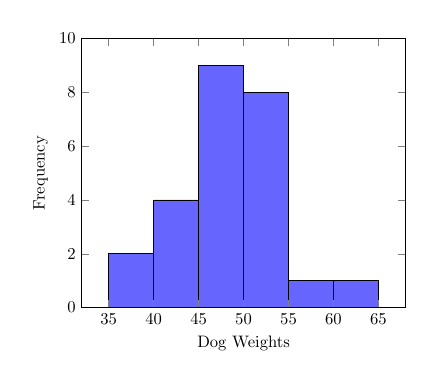
\begin{tikzpicture}[scale=0.6]
\begin{axis}[
ymin = 0, ymax = 10, area style, xlabel = {Dog Weights}, ylabel = {Frequency},
]
\addplot[ybar interval, fill=blue!60, mark=no] plot coordinates {(35,2) (40,4) (45,9) (50,8) (55,1) (60,1) (65,1)};
\end{axis}
\end{tikzpicture}
\end{center}
\pause 

Each bar is called a {\color{blue}\textbf{class}}, and in the histogram above, the class width is 5.
\end{frame}

\begin{frame}{Histograms of Quantitative Data}
\begin{minipage}{0.35\textwidth}
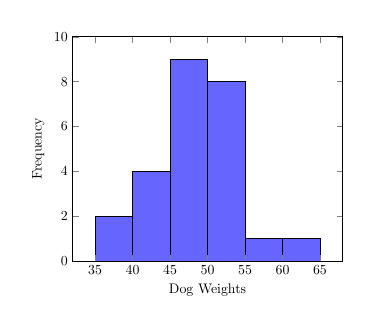
\begin{tikzpicture}[scale=0.5]
\begin{axis}[
ymin = 0, ymax = 10, area style, xlabel = {Dog Weights}, ylabel = {Frequency},
]
\addplot[ybar interval, fill=blue!60, mark=no] plot coordinates {(35,2) (40,4) (45,9) (50,8) (55,1) (60,1) (65,1)};
\end{axis}
\end{tikzpicture}
\end{minipage}
\hspace{5pt}
\begin{minipage}{0.55\textwidth}
\scalebox{0.9}{
\begin{tabular}{c|c|c}
\textbf{Class} & \textbf{Frequency} & \textbf{Class Midpoint} \\ \hline
$35 \leq x < 40$ & 2 & 37.5 \\
$40 \leq x < 45$ & 4 & 42.5 \\
$45 \leq x < 50$ & 9 & 47.5 \\
$50 \leq x < 55$ & 8 & 52.5 \\
$55 \leq x < 60$ & 1 & 57.5 \\
$60 \leq x < 65$ & 1 & 62.5 
\end{tabular}}
\end{minipage}
\end{frame}

\begin{frame}{Histogram with Class Midpoints}
\begin{center}
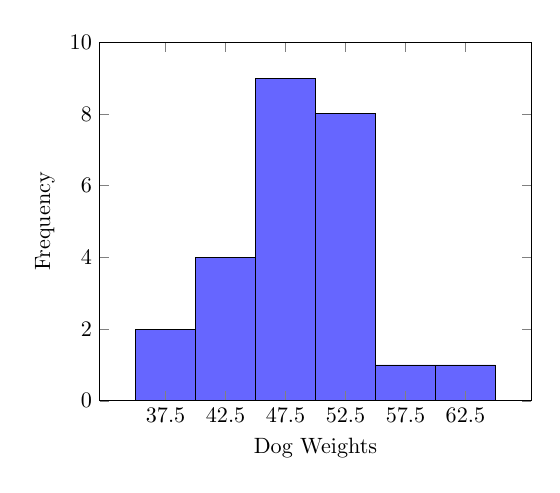
\begin{tikzpicture}[scale=0.8]
\begin{axis}[
ymin = 0, ymax = 10, area style, xlabel = {Dog Weights}, ylabel = {Frequency},
xtick = {37.5,42.5,47.5,52.5,57.5,62.5}
]
\addplot[ybar interval, fill=blue!60, mark=no] plot coordinates {(35,2) (40,4) (45,9) (50,8) (55,1) (60,1) (65,1)};
\end{axis}
\end{tikzpicture}
\end{center}
\end{frame}


\begin{frame}{Relative Frequency Histogram}
We can even make a relative frequency histogram of a data set.	\newline\\	\pause

The total area of all rectangles will equal 100\%.	\newline\\	\pause
\begin{center}
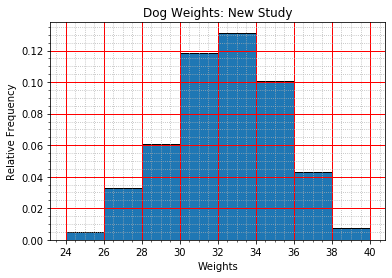
\includegraphics[scale=0.55]{../Images/dog_weights_relfreq_hist.png}
\end{center}
\end{frame}

\begin{frame}{Example 1}
Answer each given the histogram below.
\begin{center}
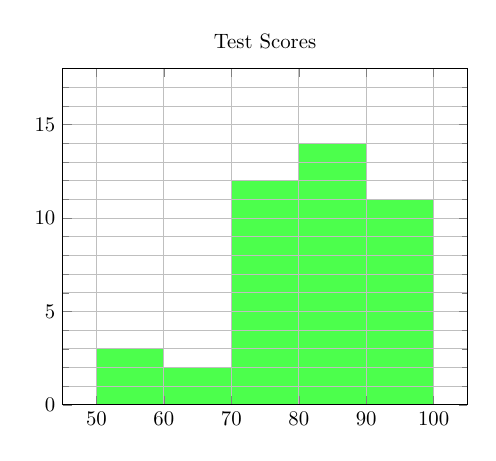
\begin{tikzpicture}[scale=0.75]
\begin{axis}[
    ymin=0, ymax=18,
    minor y tick num = 4,
    area style, grid=both, title=Test Scores
    ]
\addplot+[ybar interval,mark=no,fill=green!70] plot coordinates { (50, 3) (60, 2) (70, 12) (80, 14) (90, 11) (100, 9)};
\end{axis}
\end{tikzpicture}
\end{center}
(a) What is the class width?	\quad \onslide<2->{10}
\end{frame}

\begin{frame}{Example 1}
(b) What is the class midpoint of the 4th class?	\quad \onslide<2->{85}
\begin{center}
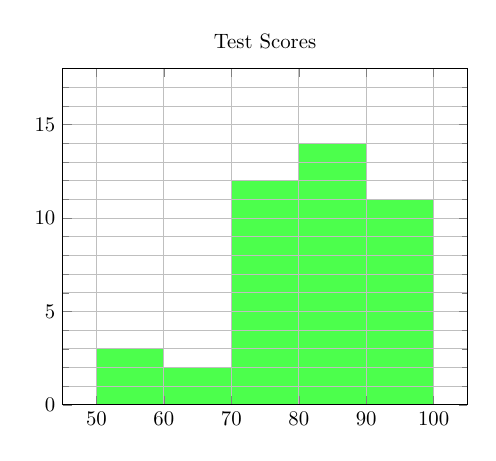
\begin{tikzpicture}[scale=0.75]
\begin{axis}[
    ymin=0, ymax=18,
    minor y tick num = 4,
    area style, grid=both, title=Test Scores
    ]
\addplot+[ybar interval,mark=no,fill=green!70] plot coordinates { (50, 3) (60, 2) (70, 12) (80, 14) (90, 11) (100, 9)};
\end{axis}
\end{tikzpicture}
\end{center}
\end{frame}

\begin{frame}{Example 1}
(c) What is the relative frequency of the 5th class?	\quad \onslide<2->{11/42}	
\begin{center}
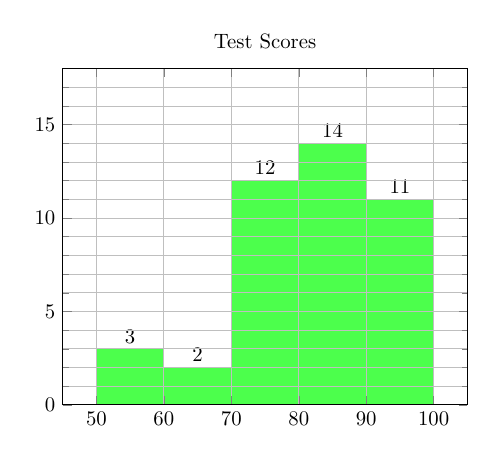
\begin{tikzpicture}[scale=0.75]
\begin{axis}[
    ymin=0, ymax=18,
    minor y tick num = 4,
    area style, grid=both, title=Test Scores
    ]
\addplot+[ybar interval,mark=no,fill=green!70] plot coordinates { (50, 3) (60, 2) (70, 12) (80, 14) (90, 11) (100, 9)};
\node at (55,3.66) {3};
\node at (65,2.66) {2};
\node at (75,12.66) {12};
\node at (85,14.66) {14};
\node at (95,11.66) {11};
\end{axis}
\end{tikzpicture}
\end{center}
\end{frame}

\begin{frame}{Example 2}
Create a histogram from the measurements below. Use the minimum value as the lower class limit of the first class and use a class width of 2.	\newline\\
\begin{center}
\begin{tabular}{ccccc}
9& 2& 10& 1& 4	\\
5& 1& 6& 7& 4	\\
6& 5& 4& 8& 10	\\ 
3& 1& 2& 3& 9	\\
8& 6& 1& 1& 10
\end{tabular}
\end{center}
\onslide<2->{Use 1,3,5,7,9, and 11 as the lower class limits.}
\end{frame}

\begin{frame}{Example 2}
\begin{center}
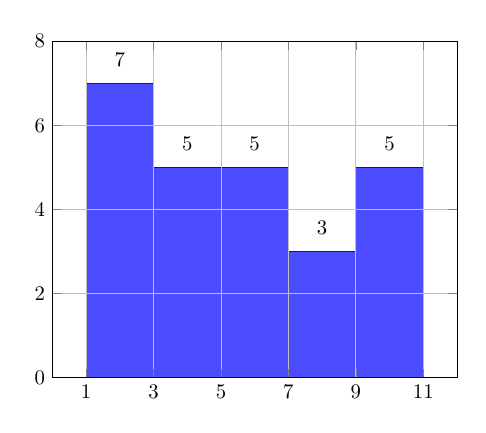
\begin{tikzpicture}[scale=0.75]
\begin{axis}[
    ymin=0, ymax=8,
    xtick = {1,3,...,11},
    % minor y tick num = 4,
    area style, grid=both, 
    ]
\addplot+[ybar interval,mark=no,fill=blue!70] plot coordinates { (1,7) (3,5) (5,5) (7,3) (9,5) (11,5)};
\node at (2,7.55) {7};
\node at (4,5.55) {5};
\node at (6,5.55) {5};
\node at (8,3.55) {3};
\node at (10,5.55) {5};
\end{axis}
\end{tikzpicture}
\end{center}
\end{frame}

\begin{frame}{Example 3}
(a) \quad Given the histogram below of the weights of 200 dogs, find the total number of dogs whose weight is at least 34 pounds.	\newline\\
\begin{minipage}{0.7\textwidth}
\begin{tikzpicture}
\node at (0,0) {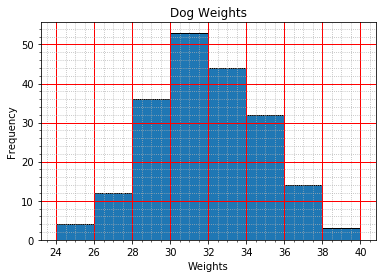
\includegraphics[scale=0.55]{../Images/dog_weights_hist.png}};
\onslide<2->{\node at (1.45,0.65) {32};}
\onslide<3->{\node at (2.15,-0.65) {14};}
\onslide<4->{\node at (2.9,-1.5) {3};}
\end{tikzpicture}
\end{minipage}
\hspace{0.25cm}
\begin{minipage}{0.2\textwidth}
\onslide<5->{Total: 49}
\end{minipage}
\end{frame}

\begin{frame}{Example 3}
(b) \quad What percentage of the dogs have weights between 26 and 28 pounds?	\newline\\
\begin{minipage}{0.7\textwidth}
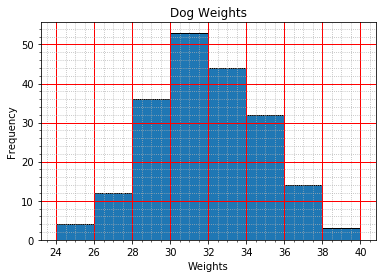
\includegraphics[scale=0.55]{../Images/dog_weights_hist.png}
\end{minipage}
\hspace{0.25cm}
\begin{minipage}{0.2\textwidth}
\onslide<2->{12/200} \\[10pt]
\onslide<3->{6\%}
\end{minipage}
\end{frame}


\begin{frame}{Some Common Histogram Shapes}
Uniform distribution:	\newline\\
\begin{center}
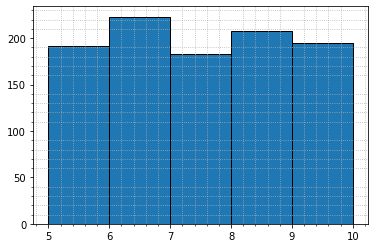
\includegraphics[scale=0.55]{../Images/uniform.png}
\end{center}
\end{frame}

\begin{frame}{Some Common Histogram Shapes}
Right (a.k.a. positively) skewed
\begin{center}
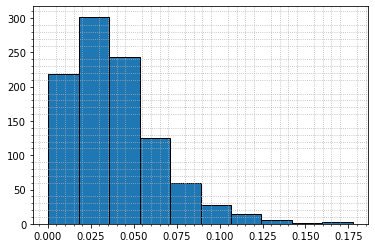
\includegraphics[scale=0.55]{../Images/positive_skewed.png}
\end{center}
\onslide<2->{\emph{Note}: Skewness refers to the \underline{tail}}
\end{frame}

\begin{frame}{Some Common Histogram Shapes}
Normal (a.k.a. bell-shaped)
\begin{center}
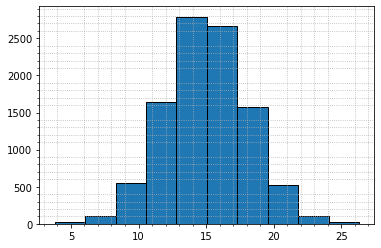
\includegraphics[scale=0.55]{../Images/normal1.png}
\end{center}
\end{frame}

\begin{frame}{Some Common Histogram Shapes}
Left (a.k.a. negatively) skewed
\begin{center}
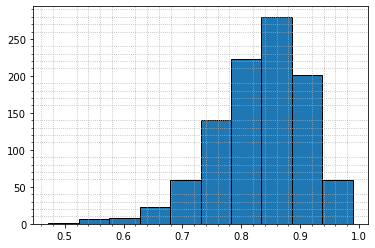
\includegraphics[scale=0.55]{../Images/negative_skewed.png}
\end{center}
\end{frame}

\begin{frame}{Cumulative Histograms}
The cumulative relative frequency histogram below shows a running total of relative frequencies of scores for a mathemathics test.
\begin{center}
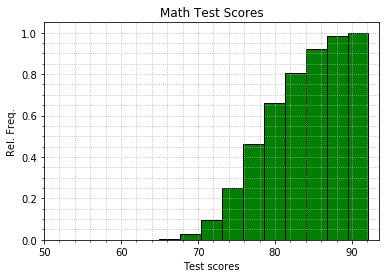
\includegraphics[scale=0.6]{../Images/cumulative_hist.png}
\end{center}
\end{frame}

\end{document}